\chapter{What is it a surface?}
\hrule
\vspace{10pt}
\begin{quote}
{ \small This introductory chapter describes the main concepts regarding the digitization of a surface at different scales, and gives an overview of the general problems the scientist may encounter. It focus on the most common techniques used, and formalize and define the terms and the concepts borrowed by different disciplines. We used the coastline mapping problem as an analogy for make acquainted the reader with the general problems. }
\end{quote}
\hrule


\section{The surface definition}
\label{sec:rapr}
The concept of surface  can be quite broad. IUPAC suggests to use this term to refer to the \textit{``outer portion'' of the sample of undefined depth}. While two different compound words are used to disambiguate the meaning and will be adopted in this dissertation, the \textbf{physical surface} defined as \textit{atomic layer of a sample which, if the sample were placed in a vacuum, is the layer ``in contact with'' the vacuum; the outermost atomic layer of a sample}
\textbf{experimental surface} \textit{That portion of the sample with which there is significant interaction with the particles or radiation used for excitation. It is the volume of sample required for analysis or the volume corresponding to the escape for the emitted radiation or particle, whichever is larger}.

In the field of nanotechnology the term \textbf{interface} is often used and can partially replace the term physical surface because in most of the application, particularly in this field, the sample is not placed in high vacuum but measured in normal atmospheric condition, and we can distinguish two o more \textbf{phases}: entities of a material system which are uniform in chemical composition and physical state. Eventually, is the definition of phase that determine the sample interface and hence our model of the boundary of the material surface. The surface unfortunately is rarely uniform and homogeneous, a more or less hydroxilized  layer is present above most of the metal and organic (check) surfaces, above this layer contaminants are usually deposited if the sample is not handle and store properly. In the field of cultural heritage we won't deal with what IUPAC define as \textbf{clean surface} but with surface where dust and grease accumulated during the century creating several interfaces.


\section{Representation of the surface}
The intent of this introduction
\subsection{Continuous representations of the surface}
The surface can be represented by \textbf{scalar-valued function} of the kind $ f(x,y) = z, \mathbb{R}^{2} \rightarrow \mathbb{R}$  
\textbf{implicit function} 
\subsection{Discrete representations of the surface}
\subsubsection*{nD array of distances}
None of the metrological instruments output directly a continuous representation of the surface but a discrete series of order value that can be eventually reshaped and stored in an array. A simple surface profile can be represented as a 1-dimensional array of the kind:
$$ P = \begin{bmatrix}
 d_{1},&  d_{2}, & \dots,& d_{i}, \\
\end{bmatrix}
$$
where $d$ is the distance from a reference line. For some applications we might want to consider the points connected and hence consider this structure as a \textbf{polygonal chain}\footnote{\textbf{Polyline} and \textbf{linestring} are terms normally found in computer science.}.\par A surface can be  represented as a 2-dimensional array, of the kind:
$$
S = \begin{bmatrix} 
    d_{1,1} & d_{1,2} & \dots \\
    \vdots & \ddots & \\
    d_{k,1} &        & d_{k,j} 
    \end{bmatrix}
$$
where $d$ still represent the distance but from a reference plane. This 2D array can produce and visualized as a 3-dimensional object, the user may be tempted to refer to this data as 2.5D ( two-and-a-half-dimensional) because it contains also information regarding the position in the third dimension, the usage of this term should be avoided because this terms is usually related to the visual perception\footnote{ three-quarter and pseudo-3D are also found in literature, the letter term even if less in vogue is actually the most preferable in the context of visual perception. An analogous concept is express by the term Trompe-l'œil in history of art.} of the data and not the data structure itself. Furthermore, the term 2.5D can be confused with the Hausdorff dimension that we encounter later on this dissertation.  We will refer to this type of data structure with the term \textbf{nD array of distances} where $n$ is one for the profiles, two for the surfaces and three for what we call surface stacks.
This representation necessitate that the distances between a measurement and the adjacent one are constant but not necessarily equal among the different axis. For instance the distance between $d_{1,n}$ and $d_{1,n+1}$ must be the same for every $n$ but it does not have to be necessarily the same of the distance between $d_{i,1}$ and  $d_{i+1,1}$. So every nD array of distance could require from one to $n$ additional terms defining what we can call \textbf{scan-step} in the context of scanning system \textbf{pixel size} for imaging systems or \textbf{sampling step} when the surface come from the sampling or discretization of a continuous signal or function \footnote{Unfortunately, often, the term lateral resolution is used, but in fact the lateral resolution can be much lower compared to the scan-step.}. A 3D array of distances can be a very handy structure for multilayer material, we can think this structure as a \textbf{surface stack} where the third dimension can be a distance but also represent time lapses. It is worth mentioning that the dimension of the array do not correspond to the dimension of the object mapped, for instance a 2D array of distance can represents portion of surface while a 3D-array of distances can represents the evolution of a surface in time so describe four dimensions. \par
The last important parameter for defining uniquely this data structure is the  \textbf{position of the reference line or plane}, in other words at what every single distance correspond. Most of the time if we output directly this data structure form an instrument the distance measured will be from the probe above the surface to the surface itself. Thus greater distances are interpreted as valleys of the surface and smaller distances as peeks. If we subtract a reference plane the interpretation will be the opposite. This may seem obvious to the operator who preform the analysis but may not be so evident for an external user of the data, and the results can be completely misinterpreted if the reference plane is taken for granted.

\begin{figure}
    \centering
    %credits to Steven B. Segletes https://tex.stackexchange.com/a/402674/33846
\setbox0=\hbox{
        \begin{tikzpicture}[every node/.style={anchor=north east,fill=white,minimum width=1.4cm,minimum height=7mm}]
        \matrix (mA) [draw,matrix of math nodes]
        {
            d_{1,1,1}  &d_{1,1,1}&  \cdots & d_{1,j,1} \\
            d_{2,1,1} &d_{1,1,1}&  \cdots & d_{2,1,1} \\
            \vdots          &  \ddots & \vdots         \\
            d_{1,2,1}  &d_{1,1,1}&  \cdots & d_{2,1,1} \\
        };
        \matrix (mB) [draw,matrix of math nodes] at ($(mA.south west)+(4.9,1.65)$)
        {
            d_{2,1}  &d_{1,1,1}&  \cdots & d_{2,1} \\
            d_{2,1} & d_{1,1,1}& \cdots & d_{2,1} \\
            \vdots          &  \ddots & \vdots         \\
            d_{2,1}  & d_{1,1,1}& \cdots & d_{2,1} \\
        };
        \matrix (mC) [draw,matrix of math nodes] at ($(mB.south west)+(4.9,1.65)$)
        {
            d_{2,1}  & d_{1,1,1}& \cdots & d_{2,1} \\
            d_{2,1} & d_{1,1,1}& \cdots & d_{2,1} \\
            \vdots     &  \vdots      &  \ddots & \vdots         \\
            d_{2,1}  & d_{1,1,1}& \cdots & d_{2,1} \\
        };
        \draw[dashed](mA.north east)--(mC.north east);
        \draw[dashed](mA.north west)--(mC.north west);
        \draw[dashed](mA.south east)--(mC.south east);
        \end{tikzpicture}%
}
\kern10pt%
\stackinset{r}{20pt}{b}{8pt}{\rotatebox{-130}{\slantbox[-.81]{$\mid\!\xleftrightarrow{~~~~~\rotatebox{180}{$\Delta y$}~~~~~}\!\mid$}}}{%
\stackinset{l}{-58pt}{b}{70pt}{\rotatebox{90}{$\mid\!\xleftrightarrow{~~~\rotatebox{-90}{$Scan~step$~~}}\!\mid$}}{%
\stackinset{c}{-65pt}{b}{-18pt}{$\mid\!\xleftrightarrow{\textstyle Scan~step}\!\mid$}{%
  \copy0
}}}
    \caption{Caption}
    \label{fig:my_label}
\end{figure}

\subsubsection*{2D and 3D arrays of generic scalars}
Large amount of analytic data can be described with the N-dimensional array (e.g. hyper-spectral or multi-spectral cubes etc. etc.). Some techniques, for instance X-ray tomography can retrieve the density of the material and hence output (after transformation of the data) a 3D arrays with scalars rappresenting densities. For retrieving the interfaces usually an algorithm (such as marching cube algorithm for 3D arrays) is used: a threshold is applied value of the scalar is used for delimiting the borders of the interface and obtaining what is called an \textbf{isosurface} (or \textbf{isoline} for 2D object). Thus the interface found depends on the threshold choose for separating the phases that the user wants to study. The output is are a series of coordinates that delimit the surface, a list of n-tuple.

\subsubsection*{List of n-tuple}
A more flexible way to represent the surface is using lists of coordinates respect to an arbitrary origin point. In a more formal way we can define it as a list of n-tuple:
 \begin{gather*}
  [(i_1, \ldots, i_n), \\
   \ldots , \\
  (i_1, \ldots, i_n)]   
 \end{gather*}
Where $n$ is two for a profile and three for a surface. This structure gives us the possibility to describe complex object where a contiunous interface have point with only one coordinate different from the other. 



\subsection{}

\section{The coastline mapping problems}
Graham, Douglas, et al. “National Ocean Service Shoreline—Past, Present, and Future.” Journal of Coastal Research, 2003, pp. 14–32. JSTOR, www.jstor.org/stable/25736597.

The reader may found useful dealing with analogous problems at macro scale before diving into the micro and nanoscale.  Historically cartographers where among the first scientists dealing with the problem of determining the boundary of interfaces. Some mathematical tools used in nanometrology have their roots in cartography.%Even if could seem off-topic in this dissertation the reader may benefit from this analogy. 
If we imagine to map the coastline of a region, we could face different problems:
\begin{itemize}
    \item How to define the water-land interface?
    \item What if the interface oscillate with time due to external factors?
    \item What instrument to use to take the measurement and at what resolution?
\end{itemize}
Beside these problems, the natural aging (in the case of the coastline, cost erosion) occurs but we consider this the phenomenon to be measured rather then a factor affecting the measurement. Hence we start dealing with each problem individually.   

\subsection{Uncertainties in determining the interface.} 
The first problem we may face is to decide where to define the water-land interface: shall we consider as boarder the wet or muddy land or only where clear water is present? Using instrumental techniques is not always possible to arbitrary choose what to consider the interface, hence the surface we are digitizing. For instance, when using an optical technique the interface detected depends on the interaction of the radiation with the material and the processing carried out by the software for reconstructing the surface. Materials transparent to the optical radiation can cause artifacts or not be detected. Furthermore, the method used for determining the interface may have less accurate results -- or artifact -- depending on the materials analyzed, the way in which we operate the instrument or the features of the surface. To overcome these uncertainties the following actions can be carried out:
\begin{itemize}
    \item Compare measurements of the same area with different techniques.
    \item Use reference standard with certified topography (and or stratigraphy).
    \item Identify materials that could be critical to acquire. 
    \item Assess the performance of the instrument and its components under different conditions and over the materials identified in the previous step.
\end{itemize}
Eventually as we saw in section \ref{sec:rapr} the surface of a material is heterogeneous and composed of various layers with different thickness, that contribute in different way to the signal collected using the instrument. In general an apriori knowledge of the material and its conservation status can help to predict uncertainties in the final output. 


\subsection{Variation of the interface due to external forces.} 
Even if we convene in the definition of the interface and we optimize our measurement procedure to identify and minimize errors and artifacts; we may experience that the interface position vary during the period of observation. The change of the position of the interface,moreover, may occur during the process of measurement compromising our survey. Coming back to the coastline mapping problem, we may experience these issues in particular during high tide or low tide of the tidal cycle.  Thus, when measuring the coastline we have also to measure the level of the tide, if the cartographer measure the tide level while performing the measuring they call these measurements \textbf{tide-coordinated} otherwise if they predict the tide level using a model (mostly based on historical records) they call these measurements \textbf{tide-predicted}.  
%cite: Advances in Mapping from Remote Sensor Imagery: Techniques and Applications
%edited by Xiaojun Yang, Jonathan LiCartographers
\par The nano-cartographer may face the same issues when measuring the surface of an object at micro or nano level. For instance, the temperature or the relative humidity may affect the positions of the interfaces, because of thermal expansions or swellings due to the absorption of moisture.
However, reaching temperature-coordinated or RH-coordinated measurements may be harder than it seems. Measuring the temperature or the RH of the object, or worse only of the environment,  would be tantamount to the cartographer involved in the coastline mapping to know the mass of the moon: if there isn't an understanding of the model governing the dynamic of the system and historical records of the object is not possible to ``coordinate'' a set of parameters to the topography of the surface measured. This is due to the fact that different equilibria are involved, and could take a lot of time to reach their stationary state  ---assuming that it exists--- at particular environmental parameters. However, if we leave the object in controlled condition for an appropriate amount of time we can create a model for estimating factor-predicted measurements.   

\section{The coastline paradox}
\begin{quote}
    ``An  embarrassing doubt arose as to whether actual frontiers were so intricate as to invalidate that otherwise promising theory'' L.F. Richardson
\end{quote}
Solving -- or mitigating --  the coastline mapping problems gives us the confidence for assessing the survey of the interface under investigation. However, when we use the final survey for calculating parameters for describing the interface (e.g. length, area, roughness \ldots) we may find a strong dependence of these parameters with:
\begin{itemize}
    \item the constraints we pose at the beginning of the measuring campaign (such as instrument, the resolution and the scan step used).
    \item the processing procedure we use to calculate them.
\end{itemize} 
The axial and lateral resolution of the instrument and the scanning step determine, up to a certain point, the computed metrological parameters of the object. In a work by Lewis F. Richardson, published posthumously in 1960, the author was trying to understand if country with a common boundary are more likely to go to war with one another compared to nations without a common boundary. To measure the coastline Richardson used a divider on printed maps of the countries. The algorithm \ref{algo:1} describes in detail the manual procedure used by Richardson.

\begin{algorithm}[H]
\vspace{5pt}
%\SetAlgoLined
\KwResult{Length of the coastline or generic profile. }
Choose the distance between the divider spikes (\texttt{the radius})\;
Choose the \texttt{direction of motion} (clock-wise or counterclockwise)\;
Choose a \texttt{starting point} on the coastline\;
Place one spike of the divider on the \texttt{starting point}\;
 \While{Intersection do not overstep the \texttt{starting point}.}{
  Find the intersections of the other spike with the border\;
  Position the spike on the first intersection found following the profile along the \texttt{direction of motion}\;
  Record that you moved the divider\;
 }
 Multiply the times you moved the divider for distance between the divider spikes.
 \caption{The procedure used by Richardson for determining the length of the coastline of the countries.}
 \vspace{5pt}
 \label{algo:1}
\end{algorithm}

The procedure can be generalized for any polygonal chain, finding the intersections of circles with radius equal to the distances between the spikes of the divider instead of the intersections with the divider. The result of this procedure applied to a profile is shown in figure \ref{fig:0_circles}. 

This an example of the  \textbf{coastline paradox} )\marginpar{Coastline paradox } \ref{} that deal with the problem that the resolution of the instrument and the method used for determining the length of a surface with irregularities at different scales influence the resulting measured length of the surface. 
%© EuroGeographics for the administrative boundaries




The coastline paradox often cause some improper direct link with the fractal geometry: in fact the coastline paradox do not imply any \textbf{self-similarity}. Hence it is most of the time impossible to predict the properties of the surface morphology at a smaller scale from a less resoluted model of the surface.  Many artificial generated surface are made trough consecutive different finishing steps causing the mixing of different patterns and micro and structure of the material.


\begin{figure}
    \centering
    % This file was created by matplotlib2tikz v0.6.17 and modifyied manually.
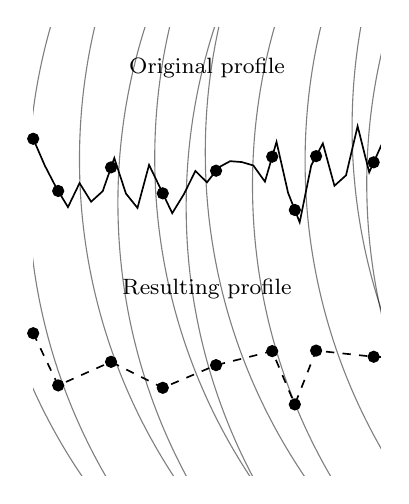
\begin{tikzpicture}

\begin{axis}[
ticks=none,
axis x line=none,
axis y line=none,
unit vector ratio*=1 1 1,
xlabel={Coordinates},
xmin=0, xmax=30,
ymin=-25.1820412260896, ymax=13.5135342876908,
tick align=outside,
tick pos=left,
x grid style={lightgray!92.026143790849673!black},
y grid style={lightgray!92.026143790849673!black}
]
\node[] at (axis cs: 15,10) {\footnotesize Original profile};
\node[] at (axis cs: 15,-9) {\footnotesize Resulting profile};
\addplot [only marks, draw=black, fill=black, colormap/viridis]
table{%
x                      y
+0.000000000000000e+00 +3.923476732411767e+00
+2.156683928570811e+00 -5.808643183291410e-01
+6.718246961960884e+00 +1.454833892983280e+00
+1.118226575965100e+01 -7.871042767195466e-01
+1.578176443460739e+01 +1.168385759481254e+00
+2.062706635908480e+01 +2.377879403103150e+00
+2.258155945158050e+01 -2.222090791109303e+00
+2.441801066199563e+01 +2.424845729208159e+00
+2.938773189705672e+01 +1.892946854622223e+00
+3.437960129517526e+01 +1.727444651252367e+00
+3.930997072173896e+01 +2.524631869890480e+00
+4.265731651955281e+01 -1.181465795078872e+00
+4.561092157751472e+01 +2.845534295781913e+00
+4.957197068064941e+01 -1.969953750689024e-01
+5.399420528914299e+01 +2.133288040044212e+00
+5.731121560736207e+01 -1.600304100976702e+00
+6.048988025170924e+01 +2.258677249904071e+00
+6.320196412883687e+01 -1.938090207008918e+00
+6.485223103478610e+01 +2.775464122665409e+00
+6.892796824021839e+01 -1.124265435031030e-01
+7.346636038123314e+01 +1.972262403602829e+00
+7.752292858743166e+01 +4.885999473215812e+00
+7.878844102989318e+01 +5.472952737330383e-02
+8.361199899648652e+01 +1.351029916813266e+00
+8.855981178051420e+01 +6.714362623091561e-01
+8.965709947755774e+01 -4.201971788642059e+00
+9.187382424709295e+01 +2.739720592077938e-01
+9.495297080758741e+01 +4.207864226135499e+00
+9.560426685112490e+01 -7.441461119598828e-01
+9.813919988718739e+01 +3.558801472869910e+00
+9.981362838761422e+01 -1.146107700064251e+00
+1.018504798611531e+02 +3.414909880915333e+00
+1.027989643971407e+02 -1.493016708667436e+00
+1.038158482771256e+02 +3.400531450006579e+00
+1.049385366369061e+02 -1.466514066148808e+00
+1.084108756650852e+02 +2.126296338332478e+00
+1.099079510422472e+02 -2.642070796798821e+00
+1.134946494337903e+02 +8.370117984669814e-01
+1.168492838971830e+02 +4.536503402023052e+00
+1.204607755568119e+02 +1.084775962632685e+00
+1.254401546012501e+02 +6.650267692975375e-01
};
\addplot [only marks, draw=black, fill=black, colormap/viridis]
table{%
x                      y
+0.000000000000000e+00 -1.285958583402084e+01
+2.156683928570811e+00 -1.736392688476175e+01
+6.718246961960884e+00 -1.532822867344932e+01
+1.118226575965100e+01 -1.757016684315215e+01
+1.578176443460739e+01 -1.561467680695135e+01
+2.062706635908480e+01 -1.440518316332945e+01
+2.258155945158050e+01 -1.900515335754191e+01
+2.441801066199563e+01 -1.435821683722444e+01
+2.938773189705672e+01 -1.489011571181038e+01
+3.437960129517526e+01 -1.505561791518024e+01
+3.930997072173896e+01 -1.425843069654212e+01
+4.265731651955281e+01 -1.796452836151148e+01
+4.561092157751472e+01 -1.393752827065069e+01
+4.957197068064941e+01 -1.698005794150151e+01
+5.399420528914299e+01 -1.464977452638839e+01
+5.731121560736207e+01 -1.838336666740931e+01
+6.048988025170924e+01 -1.452438531652853e+01
+6.320196412883687e+01 -1.872115277344152e+01
+6.485223103478610e+01 -1.400759844376719e+01
+6.892796824021839e+01 -1.689548910993571e+01
+7.346636038123314e+01 -1.481080016282977e+01
+7.752292858743166e+01 -1.189706309321679e+01
+7.878844102989318e+01 -1.672833303905930e+01
+8.361199899648652e+01 -1.543203264961934e+01
+8.855981178051420e+01 -1.611162630412345e+01
+8.965709947755774e+01 -2.098503435507466e+01
+9.187382424709295e+01 -1.650909050722481e+01
+9.495297080758741e+01 -1.257519834029710e+01
+9.560426685112490e+01 -1.752720867839249e+01
+9.813919988718739e+01 -1.322426109356269e+01
+9.981362838761422e+01 -1.792917026649685e+01
+1.018504798611531e+02 -1.336815268551727e+01
+1.027989643971407e+02 -1.827607927510004e+01
+1.038158482771256e+02 -1.338253111642602e+01
+1.049385366369061e+02 -1.824957663258141e+01
+1.084108756650852e+02 -1.465676622810012e+01
+1.099079510422472e+02 -1.942513336323142e+01
+1.134946494337903e+02 -1.594605076796562e+01
+1.168492838971830e+02 -1.224655916440955e+01
+1.204607755568119e+02 -1.569828660379992e+01
+1.254401546012501e+02 -1.611803579713506e+01
};
\draw[draw=black,draw opacity=0.5,fill opacity=0] (axis cs:0,3.92347673241177) circle (50);
\draw[draw=black,draw opacity=0.5,fill opacity=0] (axis cs:2.15668392857081,-0.580864318329141) circle (50);
\draw[draw=black,draw opacity=0.5,fill opacity=0] (axis cs:6.71824696196088,1.45483389298328) circle (50);
\draw[draw=black,draw opacity=0.5,fill opacity=0] (axis cs:11.182265759651,-0.787104276719547) circle (50);
\draw[draw=black,draw opacity=0.5, fill opacity=0] (axis cs:15.7817644346074,1.16838575948125) circle (50);
\draw[draw=black,draw opacity=1,fill opacity=0,thick,] (axis cs:20.6270663590848,2.37787940310315) circle (50);
\draw[draw=black,draw opacity=0.5,fill opacity=0] (axis cs:22.5815594515805,-2.2220907911093) circle (50);
\draw[draw=black,draw opacity=0.5,fill opacity=0] (axis cs:24.4180106619956,2.42484572920816) circle (50);
\draw[draw=black,draw opacity=0.5,fill opacity=0] (axis cs:29.3877318970567,1.89294685462222) circle (50);
\draw[draw=black,draw opacity=0.5,fill opacity=0] (axis cs:34.3796012951753,1.72744465125237) circle (50);
\draw[draw=black,draw opacity=0.5,fill opacity=0] (axis cs:39.309970721739,2.52463186989048) circle (50);
\draw[draw=black,draw opacity=0.5,fill opacity=0] (axis cs:42.6573165195528,-1.18146579507887) circle (50);
\draw[draw=black,draw opacity=0.5,fill opacity=0] (axis cs:45.6109215775147,2.84553429578191) circle (50);
\draw[draw=black,draw opacity=0.5,fill opacity=0] (axis cs:49.5719706806494,-0.196995375068902) circle (50);
\draw[draw=black,draw opacity=0.5,fill opacity=0] (axis cs:53.994205289143,2.13328804004421) circle (50);
\draw[draw=black,draw opacity=0.5,fill opacity=0] (axis cs:57.3112156073621,-1.6003041009767) circle (50);
\draw[draw=black,draw opacity=0.5,fill opacity=0] (axis cs:60.4898802517092,2.25867724990407) circle (50);
\draw[draw=black,draw opacity=0.5,fill opacity=0] (axis cs:63.2019641288369,-1.93809020700892) circle (50);
\draw[draw=black,draw opacity=0.5,fill opacity=0] (axis cs:64.8522310347861,2.77546412266541) circle (50);
\draw[draw=black,draw opacity=0.5,fill opacity=0] (axis cs:68.9279682402184,-0.112426543503103) circle (50);
\draw[draw=black,draw opacity=0.5,fill opacity=0] (axis cs:73.4663603812331,1.97226240360283) circle (50);
\draw[draw=black,draw opacity=0.5,fill opacity=0] (axis cs:77.5229285874317,4.88599947321581) circle (50);
\draw[draw=black,draw opacity=0.5,fill opacity=0] (axis cs:78.7884410298932,0.0547295273733038) circle (50);
\draw[draw=black,draw opacity=0.5,fill opacity=0] (axis cs:83.6119989964865,1.35102991681327) circle (50);
\draw[draw=black,draw opacity=0.5,fill opacity=0] (axis cs:88.5598117805142,0.671436262309156) circle (50);
\draw[draw=black,draw opacity=0.5,fill opacity=0] (axis cs:89.6570994775577,-4.20197178864206) circle (50);
\draw[draw=black,draw opacity=0.5,fill opacity=0] (axis cs:91.873824247093,0.273972059207794) circle (50);
\draw[draw=black,draw opacity=0.5,fill opacity=0] (axis cs:94.9529708075874,4.2078642261355) circle (50);
\draw[draw=black,draw opacity=0.5,fill opacity=0] (axis cs:95.6042668511249,-0.744146111959883) circle (50);
\draw[draw=black,draw opacity=0.5,fill opacity=0] (axis cs:98.1391998871874,3.55880147286991) circle (50);
\draw[draw=black,draw opacity=0.5,fill opacity=0] (axis cs:99.8136283876142,-1.14610770006425) circle (50);
\draw[draw=black,draw opacity=0.5,fill opacity=0] (axis cs:101.850479861153,3.41490988091533) circle (50);
\draw[draw=black,draw opacity=0.5,fill opacity=0] (axis cs:102.798964397141,-1.49301670866744) circle (50);
\draw[draw=black,draw opacity=0.5,fill opacity=0] (axis cs:103.815848277126,3.40053145000658) circle (50);
\draw[draw=black,draw opacity=0.5,fill opacity=0] (axis cs:104.938536636906,-1.46651406614881) circle (50);
\draw[draw=black,draw opacity=0.5,fill opacity=0] (axis cs:108.410875665085,2.12629633833248) circle (50);
\draw[draw=black,draw opacity=0.5,fill opacity=0] (axis cs:109.907951042247,-2.64207079679882) circle (50);
\draw[draw=black,draw opacity=0.5,fill opacity=0] (axis cs:113.49464943379,0.837011798466981) circle (50);
\draw[draw=black,draw opacity=0.5,fill opacity=0] (axis cs:116.849283897183,4.53650340202305) circle (50);
\draw[draw=black,draw opacity=0.5,fill opacity=0] (axis cs:120.460775556812,1.08477596263269) circle (50);
\draw[draw=black,draw opacity=0.5,fill opacity=0] (axis cs:125.44015460125,0.665026769297537) circle (50);
\addplot [semithick, black, forget plot]
table {%
0 3.92347673241177
1 1.61311657796861
2 -0.322018506189537
3 -1.97404379366261
4 0.0963368044814079
5 -1.50917730588363
6 -0.598597052088473
7 2.26035126767286
8 -0.799716790025982
9 -2.046459677215
10 1.67060268102567
11 -0.405424395890937
12 -2.49950877882407
13 -0.86679755405796
14 1.14300906585366
15 0.163319812882958
16 1.44895766247769
17 1.99168387460313
18 1.91304857194032
19 1.621256840315
20 0.225699069848203
21 3.65784034496943
22 -0.747333305372005
23 -3.28320041531127
24 1.63449414794347
25 3.52523917700917
26 -0.134185901332833
27 0.768534054210504
28 5.01297739355113
29 1.02643171877736
30 3.26126239023511
31 0.528438282338291
32 1.54726645786974
33 0.282827178256821
34 2.37375314445052
35 0.671154914642683
36 5.5810546896218
37 4.08647279300908
38 1.99451230149693
39 2.98858369887096
40 1.49182353269243
41 1.36169680211414
42 -0.0575134096225249
43 -1.76742385918949
44 1.28558969167965
45 -1.1885194467949
46 5.41470736831891
47 2.30920677395164
48 2.58088888078373
49 1.84072552929945
50 -1.72190621618574
51 3.15264664931612
52 -0.872606549392582
53 0.285193066735473
54 2.14405963432516
55 3.11027333494517
56 2.21619130937433
57 -0.477533580715864
58 -4.08522706941225
59 1.79317210219897
60 0.579111287034127
61 4.00763480275002
62 3.72988332166266
63 -1.61615508334957
64 -3.21017638561453
65 3.81331872775258
66 1.7137762104505
67 0.571693706946724
68 -0.224377999043927
69 -0.103736525889117
70 0.625270121552521
71 -1.40346621421163
72 -0.260868403772315
73 2.46042410291822
74 1.41367631095397
75 4.51720665271422
76 3.74469791221821
77 2.3190579305621
78 7.22783821978109
79 -1.86999969129212
80 -3.30080319526799
81 -0.82923996015855
82 2.86271196336441
83 -1.28493507959957
84 3.0222043300169
85 0.778372338193619
86 0.228433876009377
87 -1.58484411373113
88 2.7381769123194
89 -0.95367224475252
90 -5.89706309321679
91 0.218424844693797
92 0.2819927929383
93 0.444334592504998
94 -2.41573265328069
95 4.53473930942804
96 -4.20127758701545
97 1.65154233824183
98 3.57293256386303
99 3.4714160233065
100 -2.20380843255428
101 -0.927949072624447
102 4.17841399592788
103 -2.92006338916222
104 4.82720410699257
105 -1.87868027264006
106 2.94919289415953
107 2.45549428766776
108 2.18079810366406
109 2.04815027376572
110 -3.11756996039589
111 2.21159318436795
112 0.534806467172263
113 0.788298237096505
114 0.88677921785332
115 -1.50295959955787
116 1.89816945314986
117 5.00470892437293
118 2.69570251081447
119 0.72590176194894
120 4.80586015639174
121 -3.26983773762194
122 2.75301668143693
123 2.39629924190023
124 1.98688751477661
125 -0.932775996971157
126 2.69731843287408
127 -0.113786545816345
128 -1.7629879579416
129 0.835728458512939
130 4.07311672167327
131 4.03825028973064
132 1.68813579098031
133 0.579777691756753
134 4.01508714757245
135 0.902004241949633
136 -0.205108917673676
137 0.614482510111108
138 1.96223030748598
139 3.53171382931722
140 0.45555633371865
141 0.981333851218332
142 3.61212350079057
143 -2.41868517391541
144 2.8090241598916
145 -1.74364854406439
146 2.51531892131749
147 4.72321792525989
148 3.41800231599643
149 0.150162034160099
150 1.37517856045912
151 1.92636252625143
152 -1.2858689899996
153 -2.39442837754109
154 3.03082131499424
155 -0.571677282436496
156 4.31591250781815
157 0.837649423963761
158 4.1421264373807
159 -0.957004907774178
160 2.46652524730992
161 -1.86096708420114
162 0.931454205605837
163 6.00773696247948
164 4.18595794138008
165 2.19276271773109
166 0.649885110709844
167 -2.81390934788172
168 0.607132283815252
169 1.84327628200982
170 1.63803777825698
171 -1.36908283123454
172 -1.73266478512907
173 -2.32290712470182
174 0.338274276607017
175 7.51353428769077
176 3.01066129930091
177 2.07817417373274
178 -2.55509530365663
179 3.66662803274688
180 5.75538925800423
181 0.929472433468653
182 0.616648046115636
183 -1.08805327579992
184 0.641543095914742
185 0.134127144783255
186 2.61835353350099
187 -3.88702905559171
188 -1.71289592739662
189 1.93446089165564
190 1.64419796371208
191 0.717238834086526
192 0.359480962195007
193 -1.67538903758566
194 2.99970484556822
195 0.207317604329183
196 1.23518127235646
197 0.254038986001258
198 2.44478365281315
199 -0.0167176572709378
200 1.56731153160128
201 0.333962743371634
202 2.45802492927189
203 4.46152719721537
204 -2.83176671149749
205 0.850852329212331
206 2.9225396916151
207 2.70015037502886
208 -1.4876720986097
209 2.97387072002664
210 1.19527547649356
211 -2.58034975273063
212 0.656741099326681
213 1.04459317338699
214 -0.281050112697665
215 2.28515080994052
216 -0.75584319975271
217 -1.48768278371982
218 2.3750420269403
219 -5.49569824048798
220 1.37618060868353
221 3.28054338168078
222 1.95055413841811
223 2.91423651934991
224 0.887093197868333
225 -1.13118909932655
226 -0.397731182388892
227 1.02817572018863
228 0.980442283778038
229 1.02249031608602
230 4.85237919159652
231 0.229617874295965
232 2.82947109730124
233 4.17202948256398
234 1.15830573309593
235 -0.548493381658609
236 3.29718221387465
237 2.19573787303135
238 -0.668893728054213
239 1.38223620850355
240 -1.79509072940977
241 0.617531603814267
242 -1.13342070923767
243 -2.03335320462331
244 5.33857862962607
245 -1.92301867755878
246 1.1168346485626
247 1.50367735624524
248 -0.0250566911830821
249 3.90742449277526
250 -0.327533465668137
251 4.81865980578339
252 1.78463840549623
253 -1.11762076822682
254 5.12865867201258
255 4.28655144972156
256 1.99590191795308
257 -0.866572893807958
258 0.536281252442013
259 0.560810823750288
260 5.53852902289019
261 -3.20439656149638
262 -1.28314020639817
263 -0.362130090498508
264 -0.351719711196287
265 -1.90285698327179
266 5.15838587709117
267 -1.65173894121476
268 1.61853048699089
269 -1.7902423297423
270 0.680999057707908
271 3.39993323511476
272 1.45914333178369
273 0.172714911777537
274 0.531663529283259
275 2.01115113212924
276 1.29880829018821
277 5.28266492961433
278 -0.285274883998289
279 -0.218659459772488
280 2.68239048285274
281 3.98754264782779
282 4.4244192586937
283 0.153567453411655
284 -0.531382530015706
285 -3.28475965585662
286 2.38285704278276
287 -2.49200033924998
288 -0.487331990776679
289 1.74204199978458
290 -1.99248319206694
291 5.19039796334556
292 3.66820700667613
293 0.696598498356507
294 2.76855016216334
295 -2.90332443856221
296 -2.82798420742332
297 0.479563124720705
298 -3.44020225668711
299 -0.165180558398381
};
\addplot [semithick, black, dashed, forget plot]
table {%
0 -12.8595858340208
2.15668392857081 -17.3639268847617
6.71824696196088 -15.3282286734493
11.182265759651 -17.5701668431522
15.7817644346074 -15.6146768069513
20.6270663590848 -14.4051831633295
22.5815594515805 -19.0051533575419
24.4180106619956 -14.3582168372244
29.3877318970567 -14.8901157118104
34.3796012951753 -15.0556179151802
39.309970721739 -14.2584306965421
42.6573165195528 -17.9645283615115
45.6109215775147 -13.9375282706507
49.5719706806494 -16.9800579415015
53.994205289143 -14.6497745263884
57.3112156073621 -18.3833666674093
60.4898802517092 -14.5243853165285
63.2019641288369 -18.7211527734415
64.8522310347861 -14.0075984437672
68.9279682402184 -16.8954891099357
73.4663603812331 -14.8108001628298
77.5229285874317 -11.8970630932168
78.7884410298932 -16.7283330390593
83.6119989964865 -15.4320326496193
88.5598117805142 -16.1116263041234
89.6570994775577 -20.9850343550747
91.873824247093 -16.5090905072248
94.9529708075874 -12.5751983402971
95.6042668511249 -17.5272086783925
98.1391998871874 -13.2242610935627
99.8136283876142 -17.9291702664969
101.850479861153 -13.3681526855173
102.798964397141 -18.2760792751
103.815848277126 -13.382531116426
104.938536636906 -18.2495766325814
108.410875665085 -14.6567662281001
109.907951042247 -19.4251333632314
113.49464943379 -15.9460507679656
116.849283897183 -12.2465591644096
120.460775556812 -15.6982866037999
125.44015460125 -16.1180357971351
};
\end{axis}

\end{tikzpicture}
    \caption{Example of the generalization of the procedure used by Richardson in his classical paper on a generic profile. Notice that the bold circle intersects the profile in many points, in this case the first intersection found following the profile along the \texttt{direction of motion} is used. }
    \label{fig:0_circles}
\end{figure}
The information acquired scanning the surface determine the \textbf{level of detail} \marginpar{Level of Detail} of the scan.

\section{An ontology of object shapes}
Looking at figure it can be seen that artworks have a plethora of shapes. A classification of their shapes is relevant for choosing the right tool, evaluating the time and the requirements for its analysis. In table 

 

\begin{table}[]
\centering
\label{tab:artworkshapes}
\begin{tabular}{cccc}
\textbf{Category}                & \textbf{Sub-Category} & \textbf{Description} & \textbf{Example}
\\
\hline
\\
Flat object             &              &   Asperities under the millimeter. & Most paintings           \\
Curved object           &              & Curvature higher then xx  mm & Russian Icon            \\
Stiacciato              &              &            & \\
\multirow{3}{*}{Relief} & Low-relief   & Elements are flatten and distorted       & \\
                        &              &    Less 50\% of the depth is shown          & \\
                        & High-relief  & More 50\% of the depth is shown.              & \\
Tutto tondo             &              &   The object has no clear background.         & Statue.
\end{tabular}
\caption{A possible subdivision of artwork shapes using the current art historina terminology.}
\end{table}
%sculpture in the round https://www.britannica.com/art/relief-sculpture#ref161321
%La Caduta degli Angeli Ribelli
%flatness two set of parallel planes where the entire surface must lay.
%so if I have the three highest peaks and the three lowest vallyes I should be able to find these two planes. 
%bpy.ops.mesh.primitive_plane_add(radius = 1.5, rotation=(0,0.5*3.14,0))
%bpy.ops.mesh.primitive_uv_sphere_add(location = (0.4,0,0))
%bpy.ops.mesh.primitive_uv_sphere_add(location = (0.7,0,0))
%bpy.ops.mesh.primitive_cylinder_add(depth = 0.7,rotation=(0,0.5*3.14,0))
\section{The mutli-scale acquistion}
Some part may be acquired at higher definition


